\documentclass[../diploma.tex]{subfiles}
 
\begin{document}
 
Я там что-то реализовал причём сделал это так-то. Щас расскажу по пунктам.

\subsection{Модификация архитектуры}
Надо было запилить две фичи: локальные и глобальные условия. 
Сначала надо понять, куда добавлять изменения, давай посмотрим на архитектурру и покажем, куда можно воткнуть условия.


% сделай, чтобы не съезжала
\begin{figure}[ht!]
  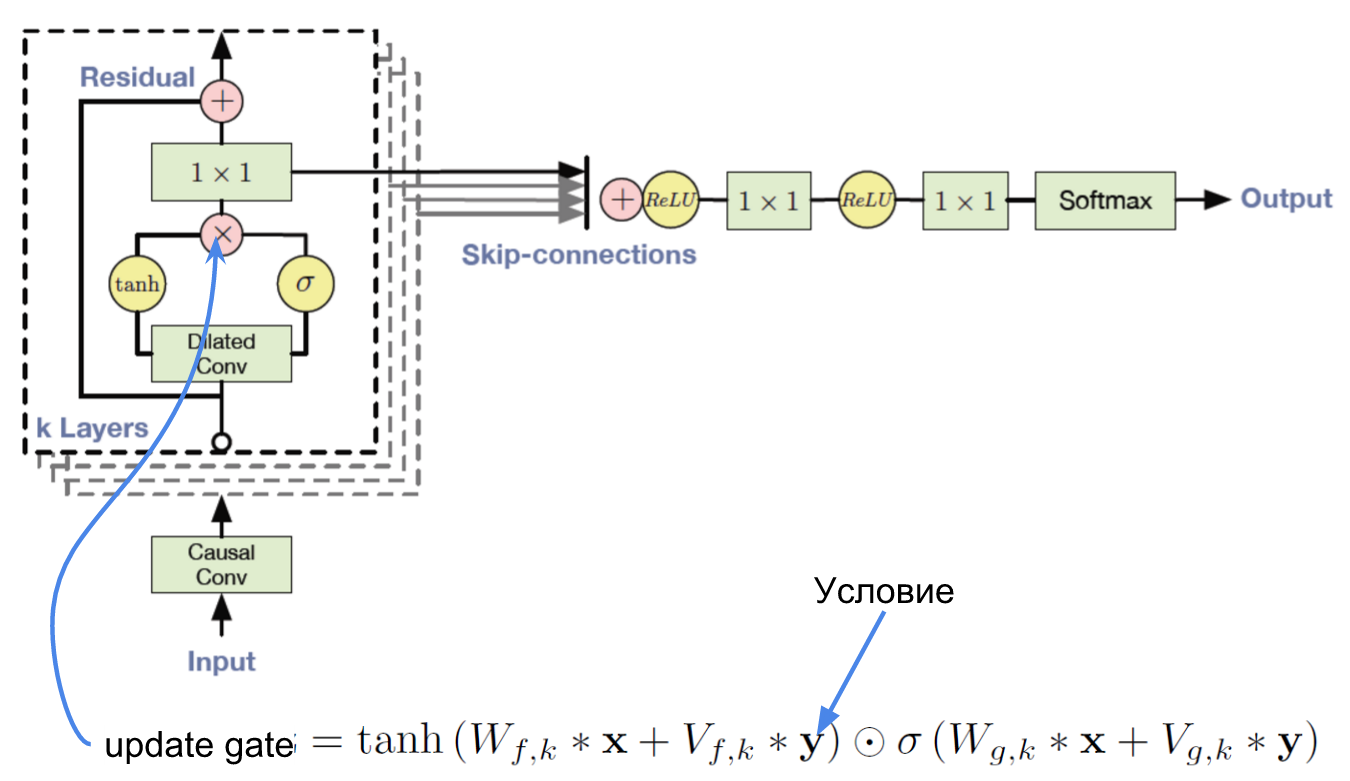
\includegraphics[scale=0.35]{img/wavenet_arrow}
  \caption{Gate, отвечающий за условия}
  \label{fig:wavenet_arrow}
\end{figure}

Ну вот видишь, условия идут в каждый гейт, поэтмоу надо добавить соотвествующие примочки в какждый dilation layer, по другому просто не получится.
По расположению они приерно одинковые, просто надо продублировать похожую штуку два раза.

\subsection{Глобальные условия}


\begin{figure}[h!]
  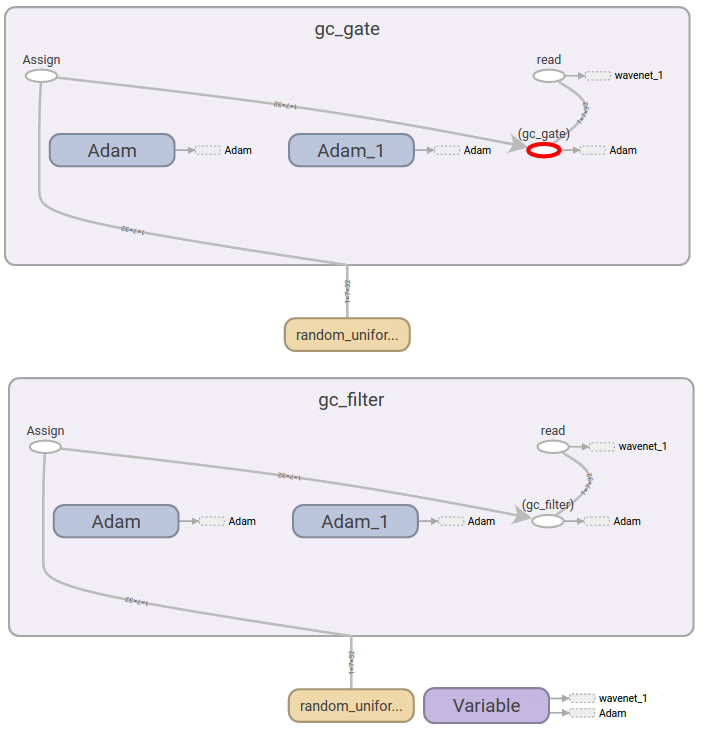
\includegraphics[scale=0.3]{img/gc}
  \caption{Глобальные условия в архитектуре}
  \label{fig:gc}
\end{figure}


\subsection{Локальные условия}




\begin{figure}[ht!]
  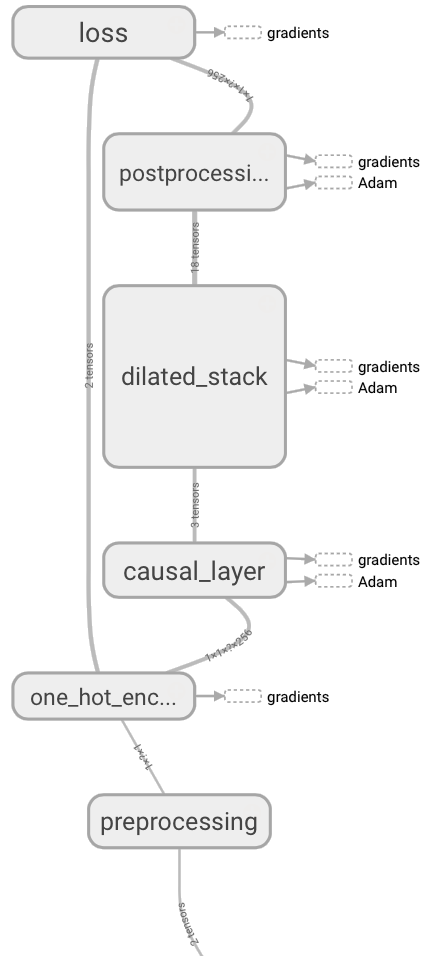
\includegraphics[scale=0.9]{img/network}
  \caption{Высокоуровневое описание архитектуры сети}
  \label{fig:arch_high}
\end{figure}


    
    % [Картиночка из tensorboard]
    
    \subsection{Generality}
    Another problem is generality: one might wish to do global coditioning where there isn't an 
    enumeration of mutually exclusive categories upon which one is conditioning. Your approach works fine
    where there are only 109 speakers in the VCTK corpus, but what if one wishes to condition upon some
    embedding vector produced by, say, seq2seq. Or a context stack (2.2 in the paper). I don't think the
    number of possible character sequences that correspond to valid sentences in a language could
    feasibly be enumerated. But you can produce a dense embedding vector of fixed size (say, 1000) that
    represents any sentence. The h in the equation at the bottom of page 4 in paper can be any vector you
    want to condition on, but with the \verb|tf.one_hot| it can only be an input to the WaveNetModel as an
    integer enumerating all possible values.
    
    \subsection{Модификаия сети}
    Здесс расскажу, как добавить туда local и global condition, потому что даже с объяснения в начале бумаги непонятно.
    
    [Картиночка из tensorboard]
    
    \subsection{Yandex-speech-kit}
    Тут на самомо деле и рассказывать особо-то нечего, налью воды про спичкит. Не зря же я столько времени просрал на это. Можно про лицензию сказать.

    % \subsection{Logging and checkpointing}

    \subsection{Реализация условий}
    
\begin{figure}[ht!]
  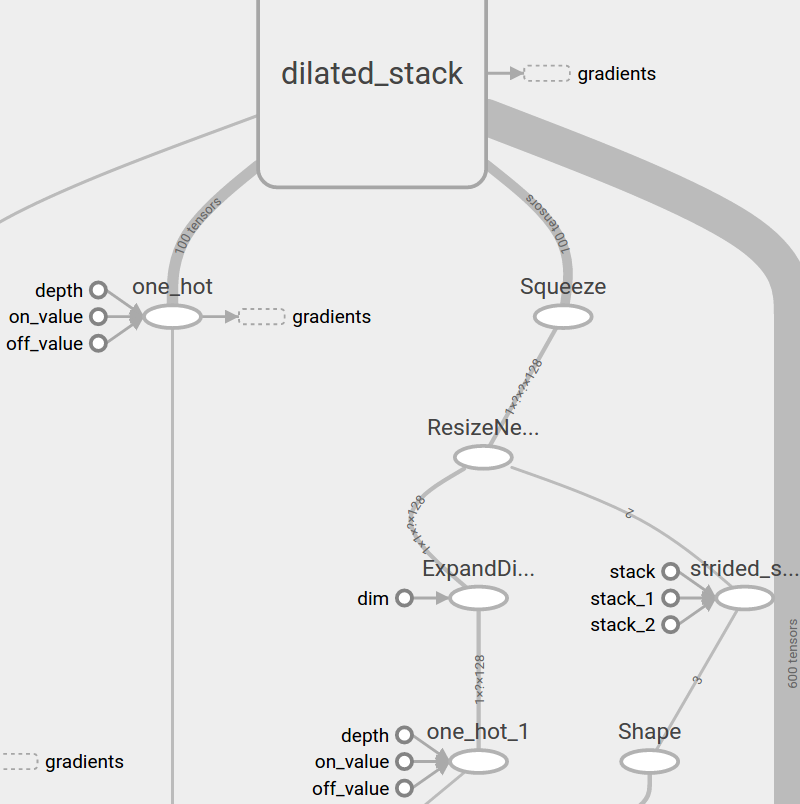
\includegraphics[scale=0.6]{img/arch}
  \caption{Низкоуровневое описание архитектуры сети}
  \label{fig:arch_low}
\end{figure}

\newpage
\pagebreak
\end{document}

